% relativeKS.tex
% copied here from nsf/nsf06am/TEX/relativeKS.tex       Nov 1 2006
% $Author$ $Date$


\subsection{\Eqva}

The KS work
% described in \refsect{s:KS}
of \refref{Christiansen:97}
was restricted to the antisymmetric subspace.
The restriction to antisymmetric subspace was used
to eliminate the continuous translational symmetry of \KSe.
Due to the lack of self-adjointness
(non-normality) of the linearized \KS\ flow, 
the antisymmetric subspace
is unstable under small perturbations, and generic solutions of 
KS belong to the full, periodic space.
Nevertheless, 
the \eqva\ and the shortest \po s orbits that lie in this subspace
and play important role for global topology of the flow,
together
with the \reqva\ and \rpo s
characteristic of the full, continuous translation invariant space..
The key new feature of the full, periodic domain
KS is its continuous translational symmetry,
with attendant continuous families of
\reqva\ (traveling waves) and \rpo s.
\Rpo s, in particular, require rethinking dynamical systems
approach to constructing symbolic dynamics. 

%%%%%%%%%%%%%%%%%%%%%%%%%%%%%%%%%%%%%%%%%%%%%%%%%%%%%%%%%%%%%%%%
\begin{figure}[t]
\begin{center} 
(a)% \includegraphics[width=0.17\textwidth]%,origin=c]
   %            {figs/kse22_E1_chaos_color.eps}
~~~
(b)%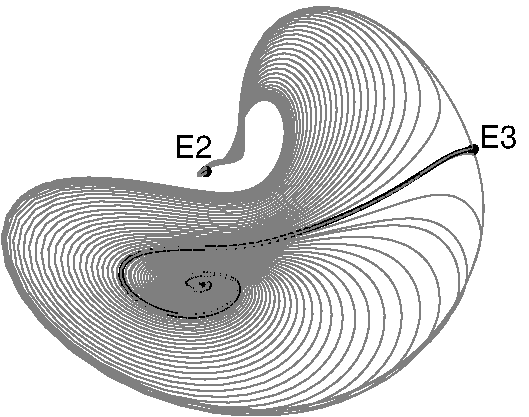
\includegraphics[width=0.33\textwidth]{figs/kse22_E1_UM2.eps}
~~~
(c)\includegraphics[width=0.3\textwidth]%,origin=c]%
        {figs/ks22E2-E3hetero.ps}
\end{center}
\caption{OBSOLETE:
(a) A perturbed unstable \EQV{1} \eqv\ and its decay
    into a typical turbulent state.
(b) \EQV{1}~\eqv\ unstable manifold, 
    with the trajectory connecting the
\EQV{2}~\eqv\ point to the unique corresponding heteroclinic
point in the \EQV{3}~\eqv\ family. 
\EQV{3}~unstable manifold in turn connects \EQV{3} to the
stable manifold of \EQV{2}.
(c) \EQV{2}~\eqv\ to \EQV{3}~\eqv\ heteroclinic 
connection. Here we omit the unstable manifold of \EQV{2},
keeping only a few neighboring trajectories in order to indicate
the unstable manifold of \EQV{3}, and show the \EQV{2} and \EQV{3}
families of \eqva\ arising from the continuous translational
symmetry of KS on a periodic domain. 
% separatrix.
% $\tilde{L}=3.5014$, 2$d$ projections from 64 
% complex Fourier modes \statesp.
        }
\label{f:KS22unstM}
\end{figure}
%%%%%%%%%%%%%%%%%%%%%%%%%%%%%%%%%%%%%%%%%%%%%%%%%%%%%%%%%%%%%%%%%%
\PC{a bit of a cheat - \reffig{f:KS22unstM} has
    2 unstable complex-pair planes}

An instructive 
example is offered by the dynamics for $L=22$ studied here.
For this small periodic cell
the chaotic dynamics arises from
a competition between unstable
wavelength 2- and 3- coherent structures.
We refer to wavelength 1-, 2- and 3- unstable \eqva\ as
\EQV{1}, \EQV{2} and \EQV{3},
respectively.
In \reffig{f:KS22unstM}(a)
color indicates the value of $u(x,t)$ in 
the $(x,t)$ space-time plane.
Spatial representations of
PDEs (such as the 3$d$
snapshots of velocity and vorticity fields in Navier-Stokes)
offer little insight into detailed dynamics of low-$Re$ flows.
Much more illuminating are the \statesp\ representations.
In \reffig{f:KS22unstM}(b) the \eqv~\EQV{1} of
\reffig{f:KS22unstM}(a) is represented by the point~\EQV{1},
and its unstable manifold can be examined in great detail.
To each \eqv\ point corresponds a continuous family
of \eqva, and this leads to an unexpected feature of such
flows: While in dimensions higher than 2 heteroclinic connections 
are a rarity (likelihood that unstable manifold of one
 \eqv\ precisely hits another \eqv\ point is zero), 
for flows with continuous symmetries intersections of unstable
manifolds with continuous families of equivalent \eqva\ are common.
\refFig{f:KS22unstM}(b) and (c) show 
such heteroclinic connections.
% from an $\EQV{2}$~\eqv\ point to $\EQV{3}$~\eqv\ family.
These connections partition the \statesp,
and will be the basis of our
{\bf construction of symbolic dynamics}.
Effective symbolic dynamics allows
for a systematic and exhaustive determination 
of all \rpo s, in the spirit of 
the earlier work. \PC{refer to it}
Many short unstable \rpo s have been already 
been computed using trial trajectories based on above
topological connections as starting  guesses 
for variants of the Newton method.


%%%%%%%%%%%%%%%%%%%%%%%%%%%%%%%%%%%%%%%%%%%%%%%%%%%%%%%%%%%%%%%%
\begin{figure}[t]
\begin{center} 
%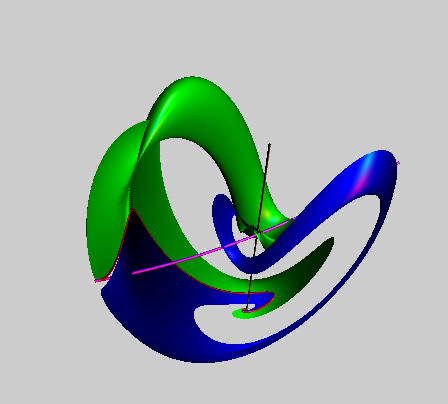
\includegraphics[width=0.6\textwidth]{figs/ks22manifold.ps}
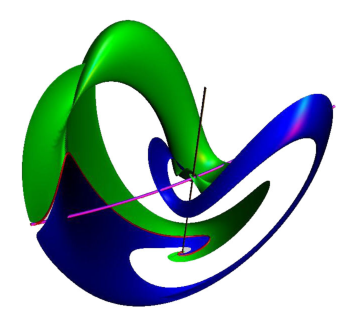
\includegraphics[height=2in]{figs/ks22manifold1.eps}
\end{center}
\caption{
    Unstable manifold of \EQV{2}~\eqv.
%\ of KS equation for $\tilde{L}=3.5014$, N=64 mode truncation.
    (black line) the family of \EQV{2}~\eqva\ 
obtained by application of the translation operator. 
(purple line) the family of \EQV{3}~\eqva.
(red) the heteroclinic connection 
from the \EQV{2}~\eqv\ to the \EQV{3}~\eqv.
The connection splits the manifold into two parts, 
colored blue and green here.
        }
\label{f:KS22Manifold}\vspace*{-5pt}
\end{figure}
%%%%%%%%%%%%%%%%%%%%%%%%%%%%%%%%%%%%%%%%%%%%%%%%%%%%%%%%%%%%%%%%%%


%%%%%%%%%%%%%%%%%%%%%%%%%%%%%%%%%%%%%%%%%%%%%%%%%%%%%%%%%%%%%%%%
\begin{figure}[t] \label{f:KS22rpo}
\begin{center} 
(a)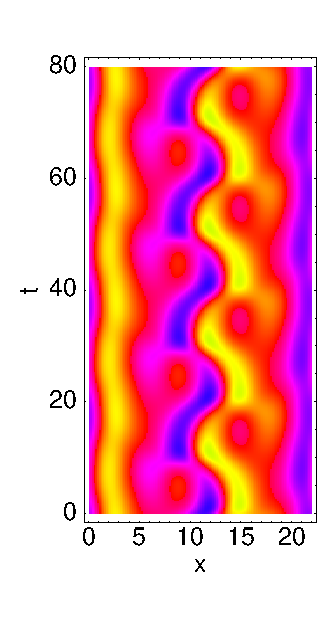
\includegraphics[width=0.2\textwidth]{figs/rpoKS21.eps}
(b)\includegraphics[width=0.2\textwidth]%,origin=c]
                {figs/rpoKS33.eps}
(c)\includegraphics[width=0.2\textwidth]%,origin=c]%
        {figs/rpoKS46.eps}
(d)\includegraphics[width=0.2\textwidth]%,origin=c]%
        {figs/rpoKS56.eps}
\end{center}
\caption{
\Rpo s of KS
equation:
% for $\tilde{L}=3.5014$, N=64 mode truncation.
(a) T=20.51, d=0.0 (\po),
(b) T=32.80, d=10.96,
(c) T=46.51, d=7.76,
(d) T=55.60, d=-5.25.
        }
\end{figure}
%%%%%%%%%%%%%%%%%%%%%%%%%%%%%%%%%%%%%%%%%%%%%%%%%%%%%%%%%%%%%%%%%%



